\section{Punktowe zagadnienie brzegowe}
%%%%%%%%%%%%%%%%%%%%%
\begin{frame}{Zagadnienie początkowe i brzegowe}
	\begin{tabular}{|l|l|}\hline
	Zagadnienie początkowe & \begin{tabular}{l}
							- ODE spełnia warunki brzegowe\\
    						w jednym punkcie - startowym
							\end{tabular}\\ \hline
    Zagadnienie brzegowe & \begin{tabular}{l}
    					- warunki brzegowe zadane w kilku\\ 
    					 punktach, zwykle na końcach przedziału 
    					\end{tabular} \\ \hline
    \end{tabular}
    \newline\newline
    \begin{block}{Przykładowo:}
    	\begin{itemize}
          \item strzałka ugięcia
          \item przepływ ciepła z T lub $\nabla T$ na brzegach
          \item drgania (membrany)
    	\end{itemize}
    \end{block}
\end{frame}
%%%%%%%%%%%%%%%%%%%%%
\begin{frame}{Przykład}
	\begin{tabular}{|l}
	Szukamy rozwiązania układu H równań różniczkowych zwyczajnych \\
    pierwszego rzędu spełniających $n_1$ warunków brzegowych w punkcie \\
    startu $x_1$ i zbiór pozostałych $n_2 = N-n_1$ warunków brzegowych \\
    w punkcie brzegowym $x_2$.
	\end{tabular}
    $$\frac{dy_i(x)}{dx}= g_i(x, y_1, y_2,\ldots, y_N)\qquad i = 1,2, \ldots, N$$
	w $x = x_1$ rozwiązanie powinno spełniać: \newline
    $$B_{1_j}(x_1, y_1, y_2,\ldots, y_N) = 0\qquad i = 1,2, \ldots, n_1 $$
	w $x = x_2$:
    $$B_{2_k}(x_2, y_1, y_2,\ldots, y_N) = 0 \qquad k = 1,2, \ldots, n_2 $$
\end{frame}
%%%%%%%%%%%%%%%%%%%%%
\begin{frame}
	\begin{block}{Twierdzenie}
		W zagadnieniach fizyki matematycznej:
        $$y'' = f(x,y,y');\qquad y(a) = A, y(b) = B$$
        jeżeli równanie jest \textbf{liniowe:}
        $$y'' = f_1(x)\cdot y'+f_2(x)\cdot y + f_3(X)$$
        to można go \textbf{sprowadzić} do zagadnienia początkowego.
	\end{block}
\end{frame}
%%%%%%%%%%%%%%%%%%%%%
\begin{frame}
	Równanie rozwiązujemy z warunkami początkowymi:
    \begin{center}
    	\begin{tabular}{ccc}
    		$y(a) = A$ & $y'(a)=\alpha_1$ & $y_1(x)$;   $y_1(b) = \beta_1$\\
        	$y(a) = A$ & $y'(a)=\alpha_2$ & $y_2(x)$;   $y_2(b) = \beta_2$
    	\end{tabular}
    \end{center}
    Wtedy funkcja zadana wzorem
    $$y(x) = \frac{1}{\beta_1-\beta_2}[(B-\beta_2)\cdot y_1(x)+(\beta_1-B)\cdot y_2(x)]$$
    spełnia równanie różniczkowe i warunki brzegowe.\newline
    \begin{block}{Rozwiązanie zagadnienia brzegowego}
    	\begin{itemize}
          \item metody strzału (shooting methods)
          \item metody relaksacyjne (relaxation methods)
    	\end{itemize}
    \end{block}
\end{frame}
%%%%%%%%%%%%%%%%%%%%%
\begin{frame}{Metoda strzału}
	\begin{figure}
		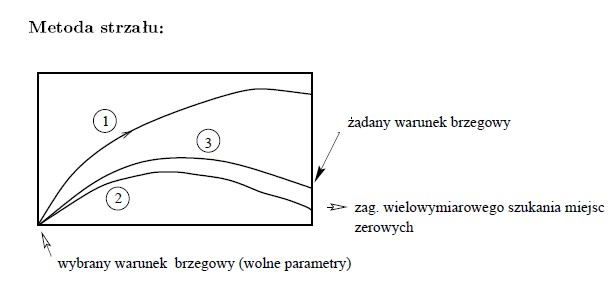
\includegraphics[height=0.55\textheight]{img/strzal.jpg}
	\end{figure} 
    Inny wariant:\newline
    \qquad rozpoczęcie całkowania ODE z obu stron, uzgodnienie parametrów przez ,,spotkanie się" rozwiązań w punkcie środkowym.
\end{frame}
%%%%%%%%%%%%%%%%%%%%%
\begin{frame}{Metoda relaksacyjna}
	\begin{figure}
		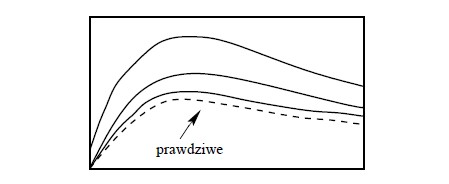
\includegraphics[height=0.35\textheight]{img/relaksacyjna.jpg}
	\end{figure}
    \begin{enumerate}
      \item równania różniczkowe $\Rightarrow$ układ równań różniczkowych
      \item iteracyjne poszukiwanie rozwiązań:
          \begin{itemize}
            \item odgadnięte
            \item po pierwszej iteracji
          \end{itemize}
    \end{enumerate}
    \begin{block}{Uwaga!}
    	Rozwiązania próbne nie muszą spełniać ani równania ani warunków brzegowych. 
    \end{block}
\end{frame}
%%%%%%%%%%%%%%%%%%%%%